% TEMPLATE for Usenix papers, specifically to meet requirements of
%  USENIX '05
% originally a template for producing IEEE-format articles using LaTeX.
%   written by Matthew Ward, CS Department, Worcester Polytechnic Institute.
% adapted by David Beazley for his excellent SWIG paper in Proceedings,
%   Tcl 96
% turned into a smartass generic template by De Clarke, with thanks to
%   both the above pioneers
% use at your own risk.  Complaints to /dev/null.
% make it two column with no page numbering, default is 10 point

% Munged by Fred Douglis <douglis@research.att.com> 10/97 to separate
% the .sty file from the LaTeX source template, so that people can
% more easily include the .sty file into an existing document.  Also
% changed to more closely follow the style guidelines as represented
% by the Word sample file. 

% Note that since 2010, USENIX does not require endnotes. If you want
% foot of page notes, don't include the endnotes package in the 
% usepackage command, below.

% F6, F11, F6, F6, F7 to compile.

% This version uses the latex2e styles, not the very ancient 2.09 stuff.
\documentclass[letterpaper,twocolumn,10pt]{article}
\usepackage{usenix,epsfig,endnotes,float}
\begin{document}

%don't want date printed
\date{}

%make title bold and 14 pt font (Latex default is non-bold, 16 pt)
\title{\Large \bf EMSS: Entity Matching in a Semi-Supervised way}




%for single author (just remove % characters)
\author{
{\rm Shaokai Wang}\\
University of Waterloo
\and
{\rm Jia R. Wu}\\
University of Waterloo
% copy the following lines to add more authors
% \and
% {\rm Name}\\
%Name Institution
} % end author

\maketitle

% Use the following at camera-ready time to suppress page numbers.
% Comment it out when you first submit the paper for review.
\thispagestyle{empty}


\subsection*{Abstract}



\section{Introduction}
Entity matching (EM), also known as Entity Resolution (ER), in the world of data management refers to resolving duplicate entities to a single entity. Matching may be done in a probabilistic or a deterministic (rule-based) manner. According to our survey, many end-to-end machine learning based methods have been applied to this problem such as Magellan, Data Tamer, JedAI to name a few. \cite{konda2016magellan, stonebraker2013data, papadakis2018jedai}.

However, traditional supervised learning methods in entity matching have a problem. They generally lack labels for training. Usually there are two ways to solve the problem: training on other labeled datasets, or labeling the training dataset manually. The first approach may fail to train a representative generalized model if the two training datasets are not similar. The second one requires a non-trivial amount of human labor. To find a good solution to this problem, we propose to use active learning, a semi-supervised learning method, to do the labeling \cite{settles2009active}.

Active learning in the context of machine learning describes the process of a user actively providing labels for model training. This paradigm of active human labeling is referred to as human-in-the-loop machine learning, which is, the model selects the most informative sample to be labeled by the human and training is conducted with these samples. We found a method called Dedupe.io which has applied active learning in entity matching, but we found that they have low recall. 

In our paper, we first provide a comparison of Entity Matching across popular packages such as Magellan and Dedupe.io \cite{bilenko2004learnable, konda2016magellan}. Comparisons are conducted with two datasets ABT\_BUY and RESTAURANTS. Additionally, we provide a fully reproducible and containerized environment for execution requiring no external dependencies other than Docker \cite{docker:2014}. Finally, we propose EMSS(Entity Matching in a Semi-Supervised way) by extending Magellan with semi-supervised learning and demonstrate that comparable accuracy for EM can be achieved with less samples.
\\

We make the following contributions:
\begin{itemize}
  \item An evaluation of EM across common systems
  \item A framework for reproducible execution
  \item An active-learning extension for EM (semi-supervised)
\end{itemize}

\section{Problem definition}
In this work, we focus on structured entity matching when resolving two csv tables. Given two structured csv tables, our aim is to combine them into a single table. During the combination, our method can detect the same entity that appears in both two csv tables and delete one of them, which is also called deduplication. After the combination, it will return a table that has information of two tables and has no duplicate entities.

\section{Related Work}
There has been much work done throughout the years to address entity matching. Efforts ranging from traditional machine learning to simple rule based entity matching have been investigated \cite{kopcke2010frameworks, fan2014emdr, elmagarmid2007survey}. Optimizations to reduce the amount of user effort in labeling with respect to a time cleaning budget have been explored \cite{ao2019cleaningem}. Other works have attempted to distribute and parallelize the blocking step \cite{chu2016distributed}. 

\subsection{Magellan}
Magellan is described as an end-to-end EM framework as it provides the user with a toolset to conduct EM from the beginning of the workflow through the end. These tools include user guides, strategies for blocking, sampling and matching. The following is a description of the Magellan workflow.

Initially, Magellan computes the cartesian product of both tables. From this resultant set of ordered pairs, an overlap blocker is applied for a resulting set C. The blocking technique used within Magellan is an overlap blocker. Attributes are tokenized into q-grams and blocked together if they share 1 minimum overlap between q-grams. Subsequently, a sample denoted by S of 450 tuples is taken from this ordered set C. Users are expected to add labels to these, denoting if they are identical entities or not.

I and J are computed from this labeled set S.

I is the training set. J is the testing set.

Feature vectors are then extracted from tables I and J. An example of a feature in this instance would be a function that maps a tuple pair into a value. If the attributes are textual, a feature could be a 3-gram jaccard score. Sample set S is thus split into training and testings sets, and six various machine learning strategies are applied to match values. The six included are Decision Tree, Support Vector Machine, Random Forest, Logistic Regression, Linear Regression and Naive Bayes. Each matcher is evaluated on the test set J and the test set I for precision and recall.

\subsection{Dedupe.io}
Dedupe.io is available as both an open source and as a paid service for EM. We will focus on the open source implementation of dedupe in this paper. The user workflow of Dedupe.io is very similar to Magellan: attributes are defined for blocking purposes and a learnable matching function is trained. However, Dedupe.io utilizes an active learning system to obtain the label: it first uses a distance matrix to find most probable same entity pairs to be labeled and then finds the most informative pairs to be labeled. Based on these labeled data, a resultant clustering component will produce a dataset with the most probable duplicates clustered together.  

According to our survey, Dedupe.io is the only EM method that applies active learning. We found that the precision of Dedupe.io is usually very high but the recall is very low when there is not sufficiently labeled data. To our understanding, the reason is that Dedupe.io uses clustering to find the same entity rather than using a classifier to judge whether it is the same entity. This will make Dedupe.io consider less pairs. 

\section{Methods}

\subsection{Docker}
Docker is a virtual-machine like system where each container (vm) offers a consistent and reproducible execution environment. Docker-compose is a standard for defining different Docker containers. By offering our code in a Git repository paired with a Docker configuration for each tool, each project can be pulled into a host machine and run + evaluated with few lines of code. Additionally, the dependencies for each tool are different, with  Magellan and Dedupe.io requiring differing numpy versions in addition to other differences. Thus, with our docker-compose setup we are able to evaluate all our tools simultaneously on a single host machine.

\subsection{Active Learning}
Active learning is a semi-supervised machine learning framework that can interactively obtain labels for training dataset. The reason we need active learning is that there are always available datasets but the labels for them are not always available. In entity matching problems, usually it is very hard to have large labeled datasets to train a machine learning model. With the same limited labeled data, if one data contains more information, it is more likely to train a stronger model. Hence, we propose Entity Matching in a Semi-Supervised way, or EMSS for brevity. We will apply active learning to improve Magellan. 

\subsection{EMSS}
EMSS divides the labeling process into several rounds. For each round, it asks a human a batch of pairs to be the same or not. At the first round, it randomly selects pairs from the whole dataset. For the next several rounds, EMSS will first use the trained model to test the whole dataset. Based on the result, there are three ways of sampling: random sampling(RS), less confident(LC) and breaking ties(BT). Random sampling is like what we do at first round: randomly select a batch of pairs. Less confident is the selection of samples which are less confident, that is, the probability value of any class is very low. Breaking ties is the boundary region selection between two classes, that is, the probability value of most probable two classes are very close.

\section{Results}
\subsection{Datasets}

\begin{figure}[H]
\centering
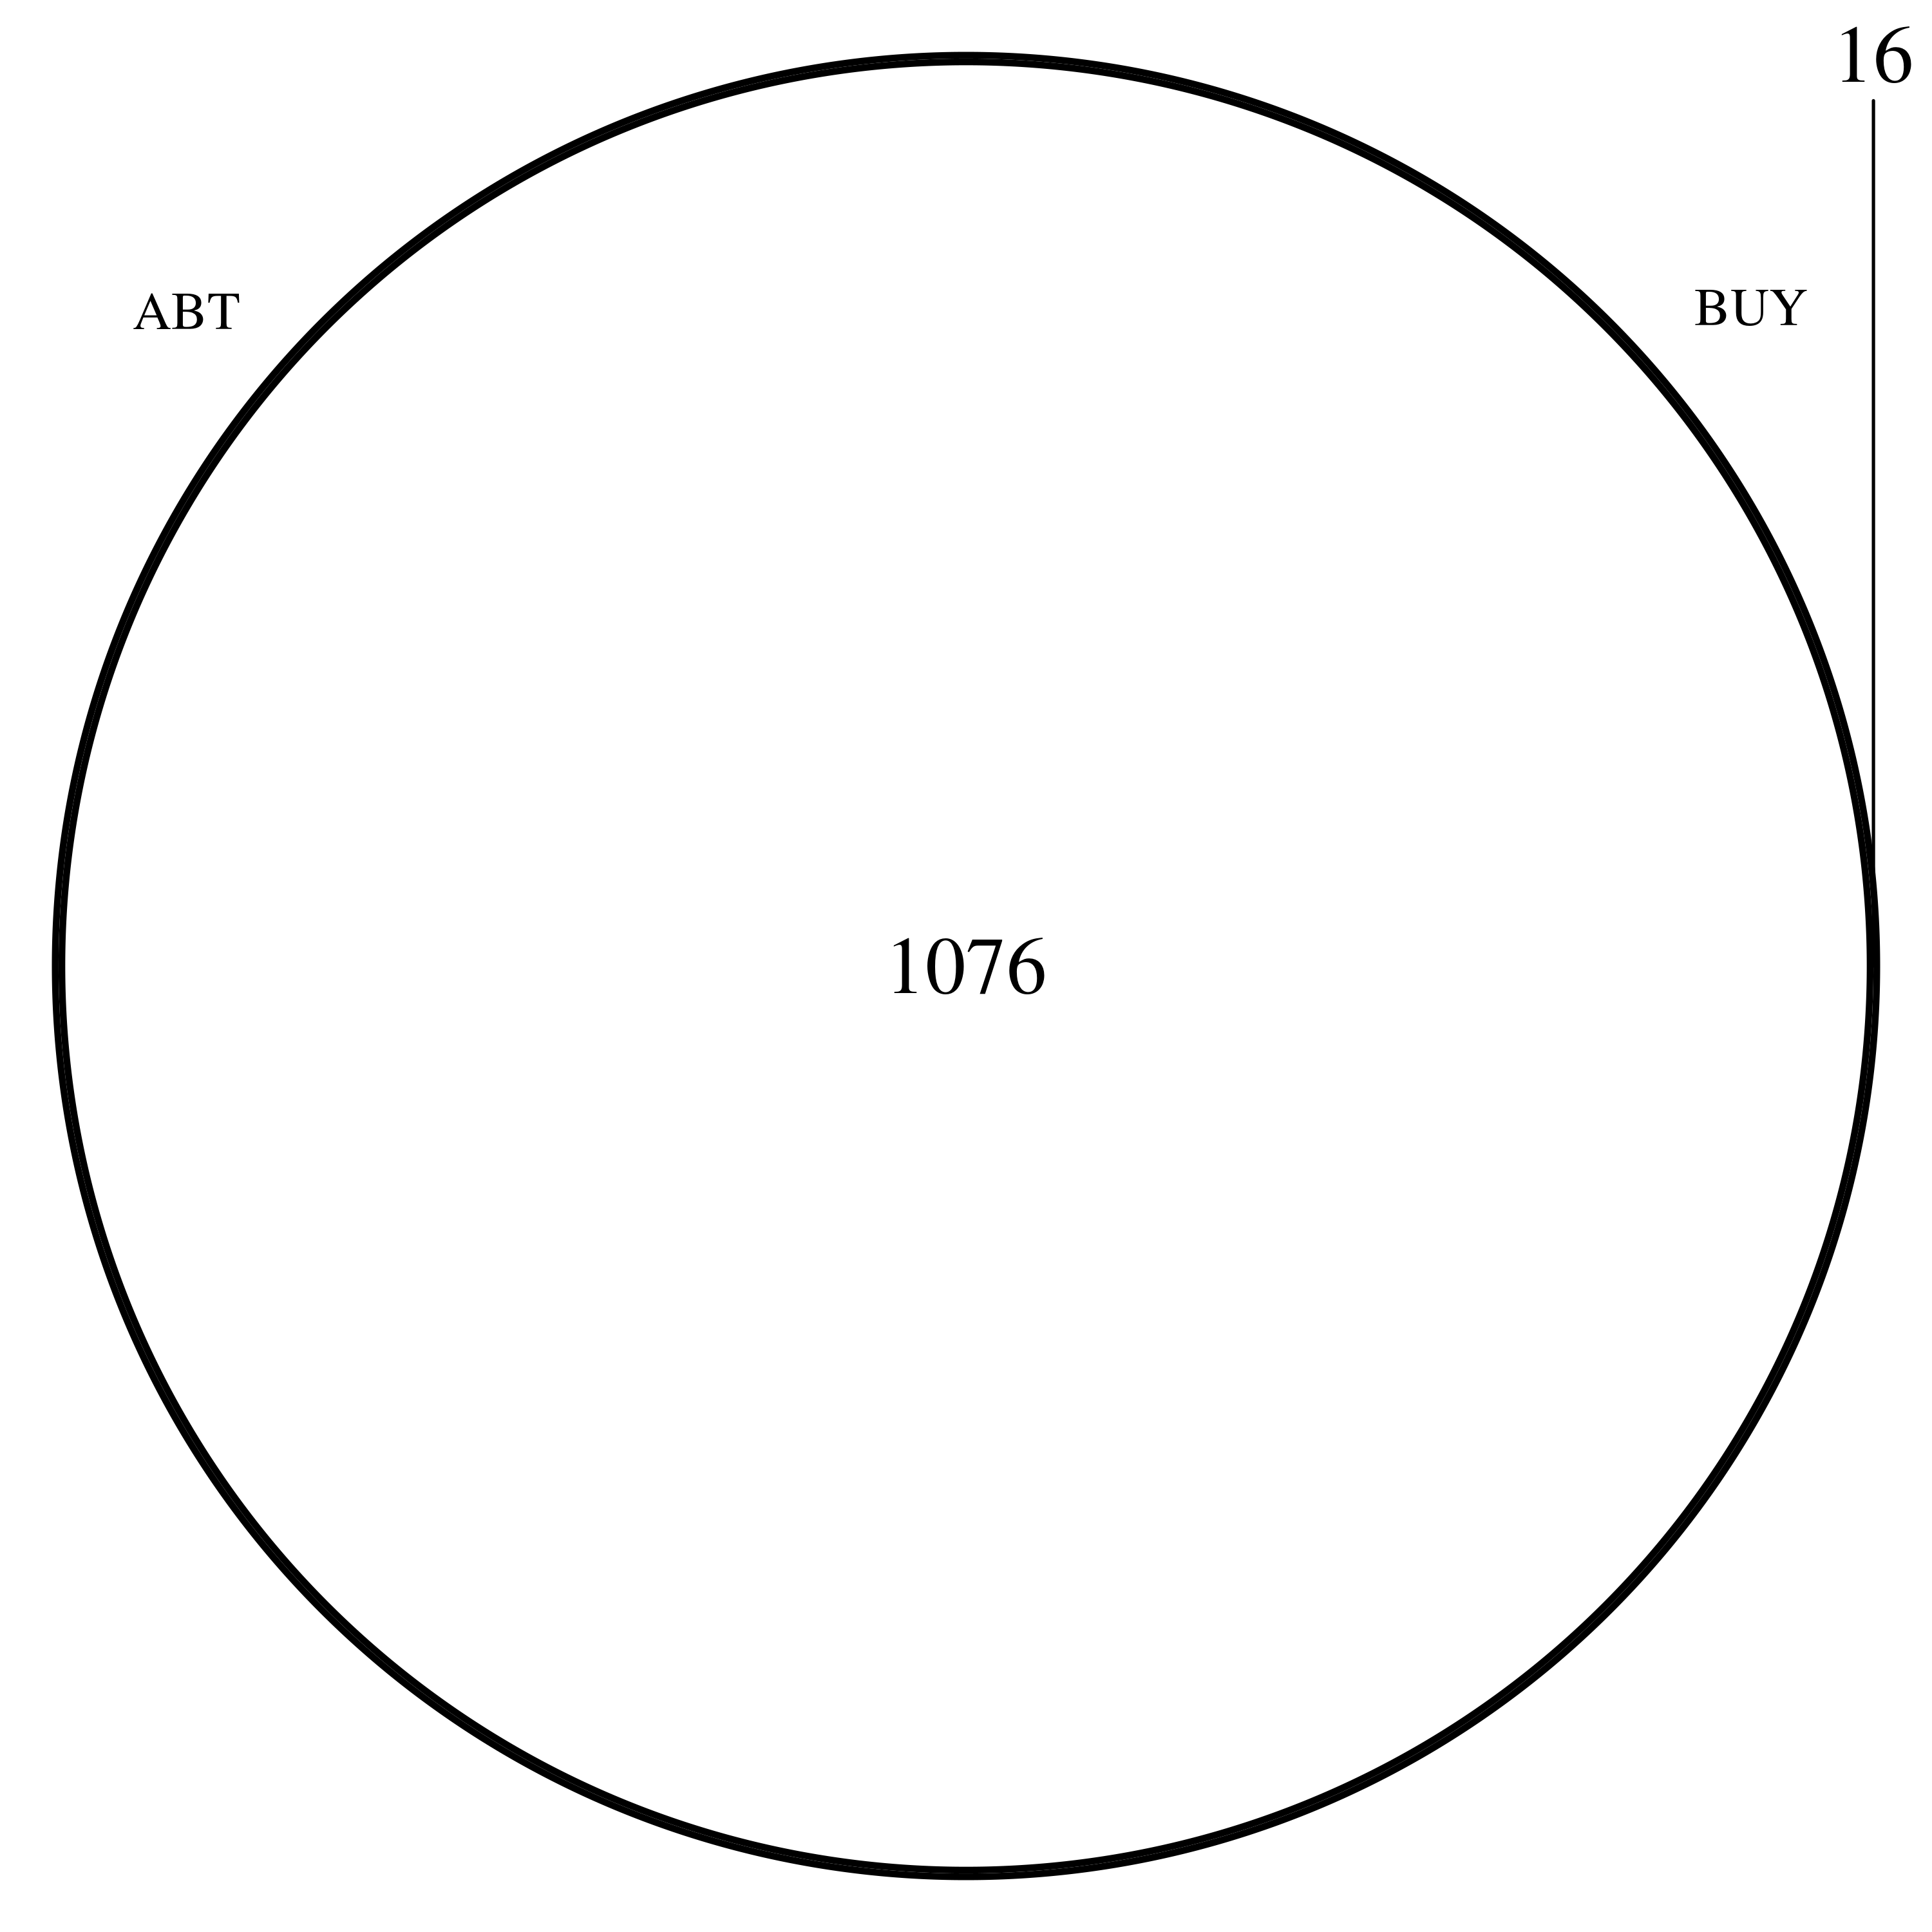
\includegraphics[width=3in]{figures/abt_buy_venn.png}
\caption{ABT\_BUY Entity Overlap}
\label{fig:abt-buy-png}
\end{figure}

The \textbf{ABT\_BUY} dataset represents two records kept of electronics. There are 4 attributes in this dataset, [\textbf{id, name, description, price}]. This is a dataset referring to electronics and their prices. Attributes name and description are highly variable and price may be absent in tuples between the two tables. As referenced by Figure \ref{fig:abt-buy-png}, ABT\_BUY primarily consists of overlapping entities. There are a total of 1076 overlapping entities between ABT and BUY with 16 entities in BUY that are not present in ABT.

\begin{figure}[H]
\centering
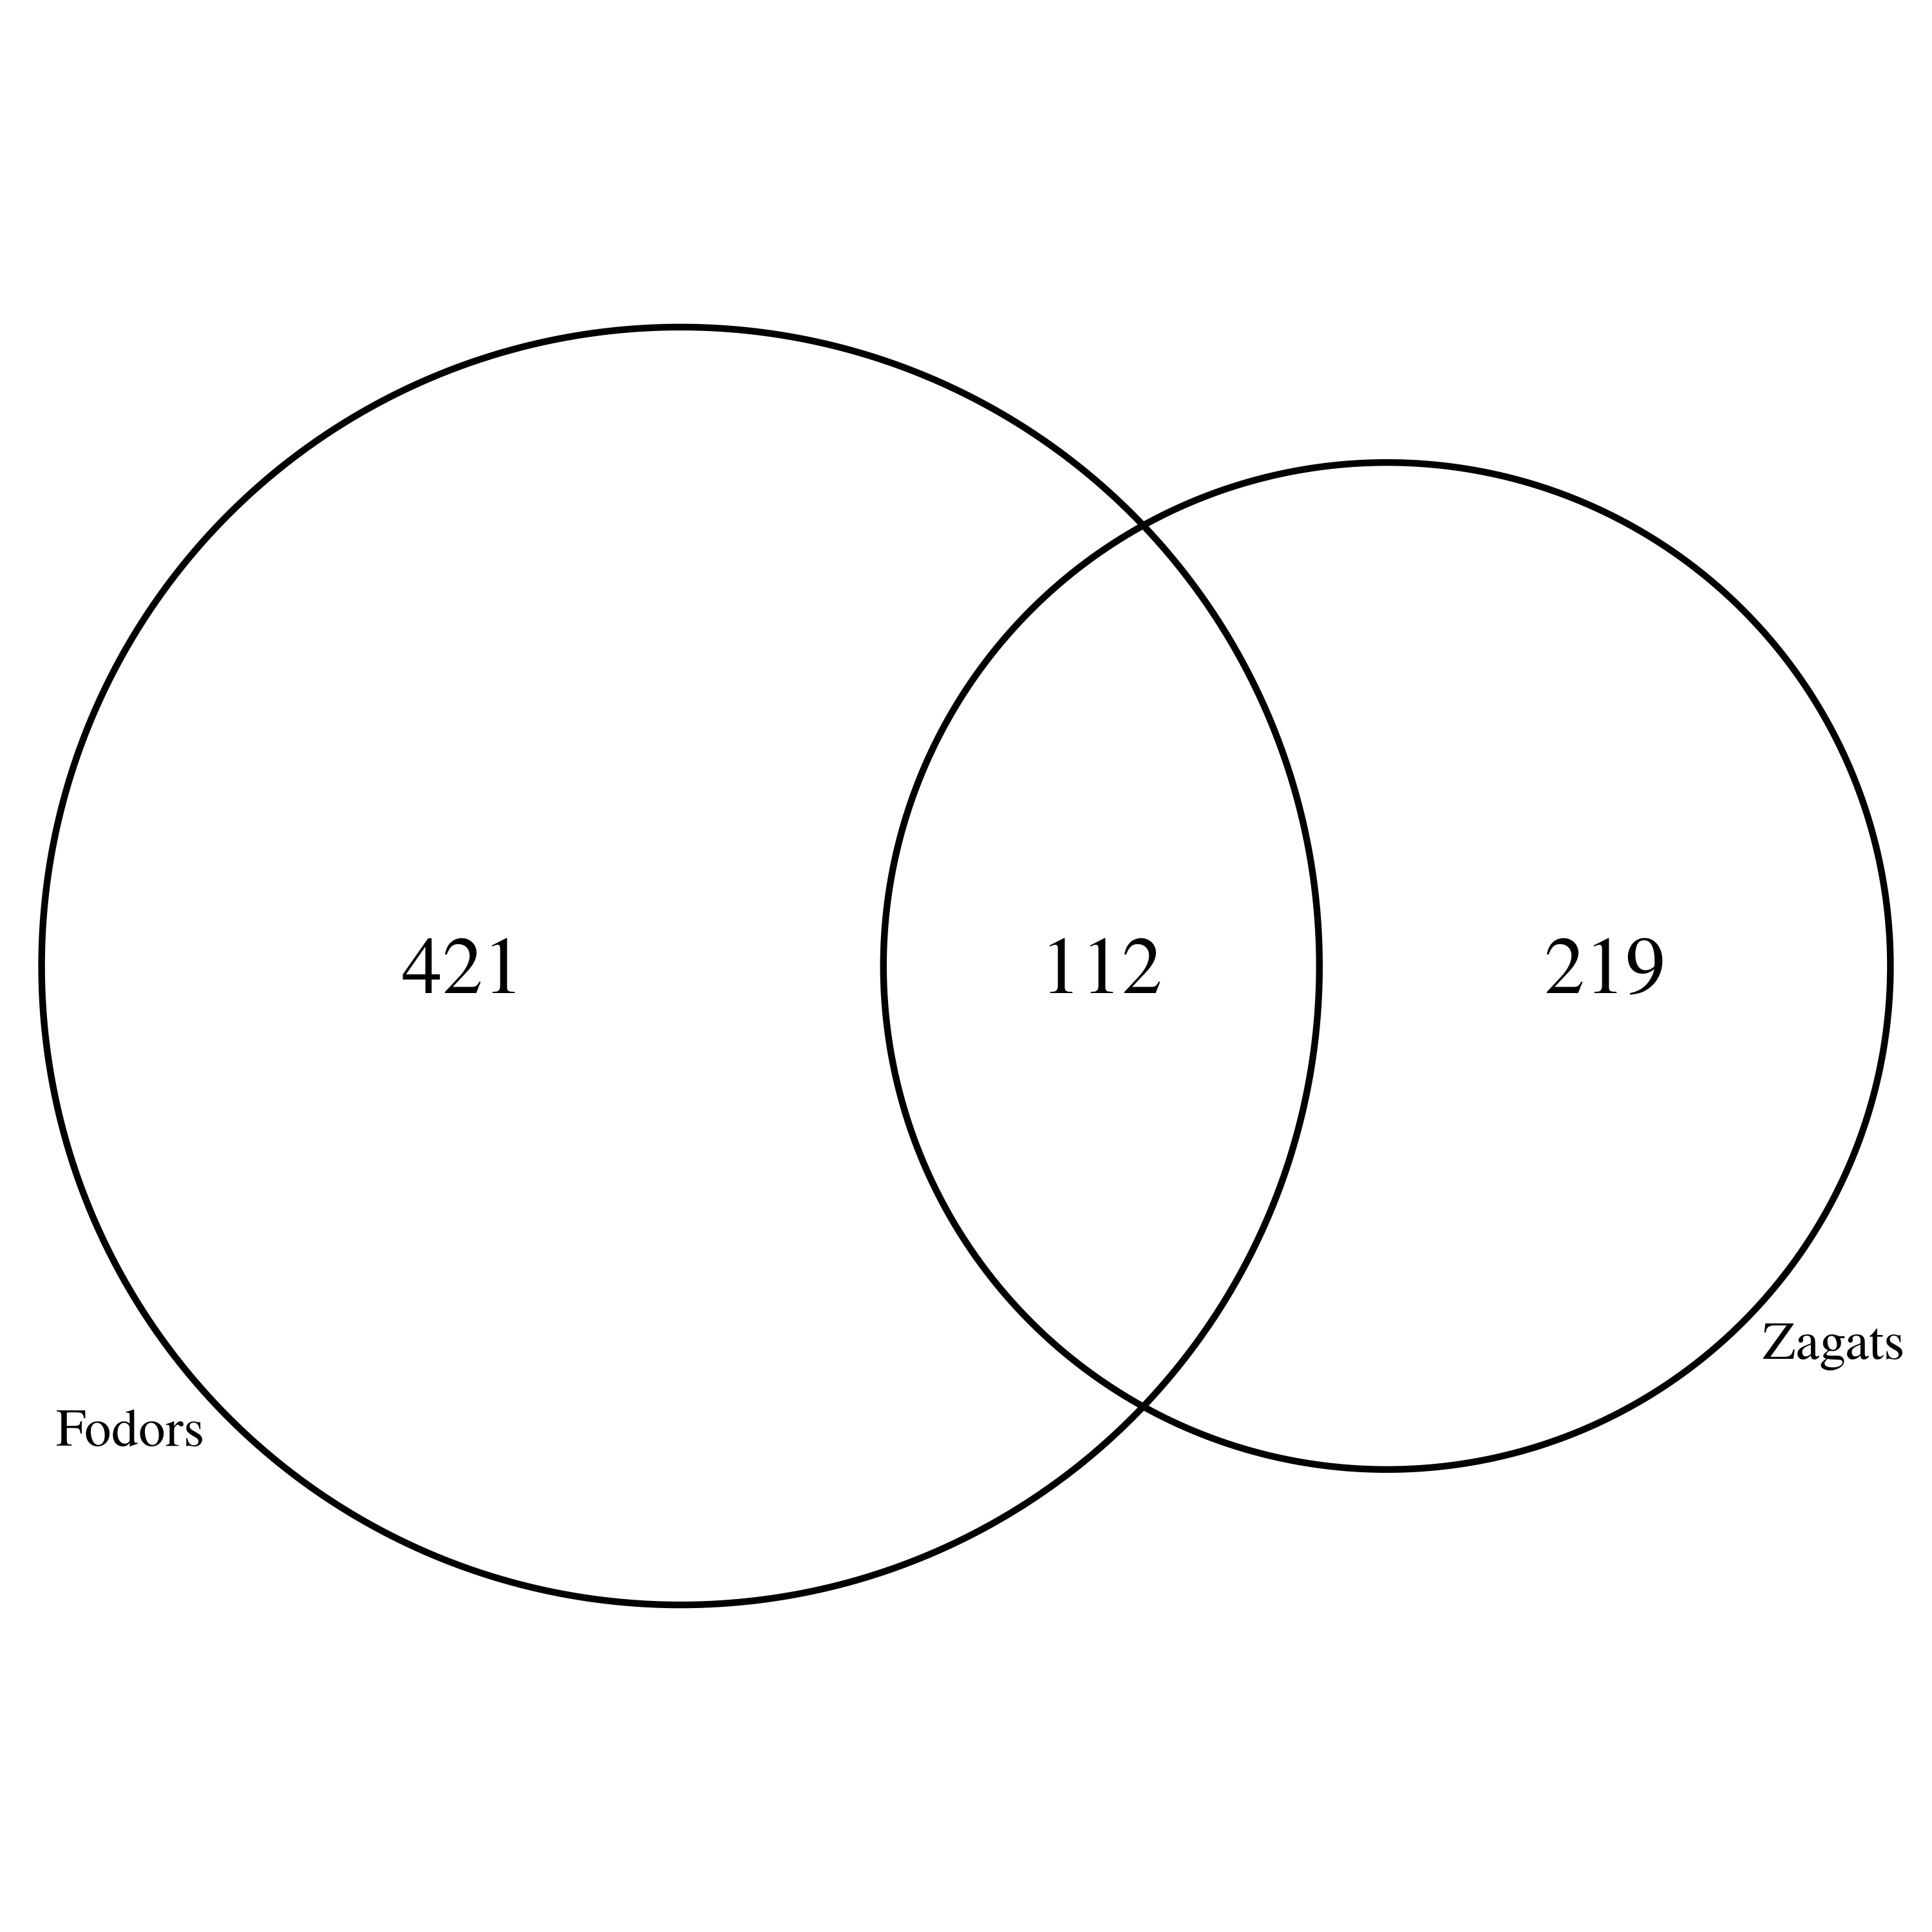
\includegraphics[width=3in]{figures/restaurants_venn.png}
\caption{Restaurants Entity Overlap}
\label{fig:restaurants-png}
\end{figure}

The \textbf{RESTAURANTS} dataset represents restaurants listed by two different review platforms. There are 6 attributes in this dataset, [\textbf{id, name, addr, city, phone, type}]. All attributes in both CSVs are present and differences are not too variable between the two. As highlighted by Figure \ref{fig:restaurants-png}, there are only 112 common entities between the two, with 421 unique entities in Fodors and 219 unique entities in Zagats.


\begin{figure}[H]
\centering
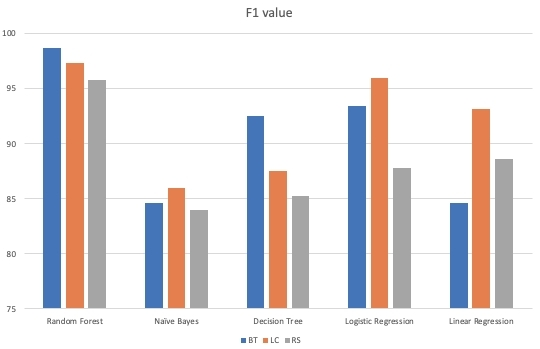
\includegraphics[width=3in]{figures/figure_1_f1.jpg}
\caption{F1 Scores of EMSS on RESTAURANTS dataset}
\label{fig:restaurants-png}
\end{figure}

This figure is a description of the F1 scores on the RESTAURANTS dataset. The batch size was 4 and the number of active learning rounds was 5. 


\noindent\fbox{
    \parbox{\columnwidth}{
    	\centering
        \textit{EMSS boosts the F1 score on all classifiers except for Linear Regression. }
    }
}
\\\\

\begin{figure}[H]
\centering
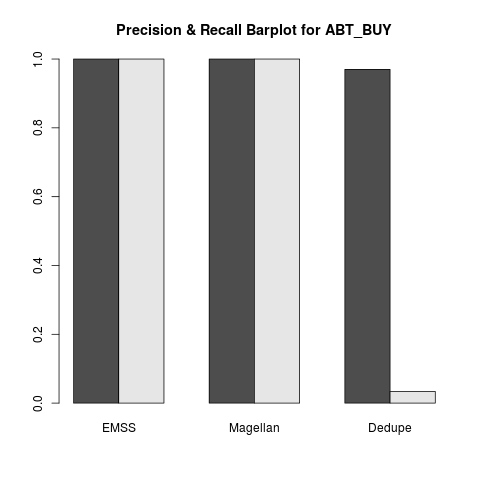
\includegraphics[width=3in]{figures/figure_2_barplot.png}
\caption{Precision vs Recall Barplot. Precision is on Left, Recall is on Right.}
\label{fig:restaurants-png}
\end{figure}

Figure \ref{fig:restaurants-png} depicts the Precision vs Recall graph for EMSS, Magellan and Dedupe.io on the ABT\_BUY dataset. Base Magellan has some strange performance where it lists both Precision and Recall as 1. \\

\noindent\fbox{
    \parbox{\columnwidth}{
    	\centering
        \textit{EMSS outperforms Dedupe.io on the ABT\_BUY dataset when a low number of training samples are used. (n=20)}
    }
}
\\\\

\section{Challenges}
Both Magellan and Dedupe.io had documentation however Dedupe.io was documented towards developers and Magellan was documented for researchers. Thus it was not clear what blocking function was used for the RecordLink class. Despite having claimed that their documentation is very good, we had to consult the libraries they used such as scikit-learn and pandas to understand what functions in Magellan did. 


\section{Threats To Validity}
As we only used two different datasets, we are unable to say that active learning works well across multiple different domains. Additionally, the entities within each dataset are known to be mostly duplicates, thus we cannot say with confidence that our method can resolve datasets where there are few duplicates better than standard Magellan or Dedupe.io. Future work would be to vary the proportion of duplicates across pairs of datasets that need to be resolved. 

We did not experiment with aggregation of multiple different blocking functions. A future direction of work would be to conduct an empirical evaluation of permutations of different blocking functions and investigate whether or not our observations change. 

The entity matcher in Magellan is the best performing matcher from one of the following: Decision Tree, Support Vector Machine, Random Forest, Logistic Regression, Linear Regression and Naive Bayes. Despite how optimized the training data selection becomes for each of these methods, the downstream matching of entities will be limited by the same drawbacks of each of the aforementioned machine learning methods. In structured data, the assumptions of these methods generally hold, however there are other methods that work better on unstructured data such as DeepER and others \cite{ebraheem2017deeper, mudgal2018deep}.

\section{Availability}\label{Availability}
All relevant scripts and data can be retireved from the following repository:
\begin{center}
{\tt https://github.com/JRWu/cs848w20}
\end{center}



{\footnotesize \bibliographystyle{acm}


\newpage
\bibliography{bibliography}}

\end{document}

